\chapter{Arquitectura}
\label{Implementación}
\section{Estructura de clases del Proyecto}
En este apartado, vamos a explicar la estructura software de este proyecto, mostrando las escenas en las que se divide el juego, las clases en las que se agrupa el código como estas se relacionan entre sí.

Sin embargo, antes de mostrar la estructura, realizaremos una pequeña exposición acerca de la forma de trabajar en Unity, hablando del lenguaje de programación usado y de los patrones de diseño en los que se basa este motor.

\subsection{Escenas}
Al igual que muchos otros motores de juegos en tres dimensiones, Unity organiza las entidades del juego haciendo uso de \textbf{Grafos de Escena}. Los Grafos de Escena son un tipo de estructura de datos que permite representar las relaciones jerárquicas que existen entre los distintos objetos del juego o ``nodos'' haciendo uso de un grafo dirigido sin hijos \cite{libro_esi}. El uso de este tipo de estructura permite gestionar con facilidad escenas tridimensionales complejas, permitiendo que se apliquen las transformaciones (traslación, rotación y escalado) y otras operaciones de un nodo padre a todos sus nodos hijos de forma automática.

La implementación de grafos de escena que Unity utiliza da soporte a la creación de multiples escenas independientes, pudiéndose realizar cambios de escenas o cargar varias escenas simultáneamente. Esto nos permite dividir el juego en múltiples secciones separadas, cada una con su propia funcionalidad. Nuestro proyecto está formado por cuatro escenas:
\begin{itemize}
  \item \textbf{Escena de Titulo}: Una sencilla escena de titulo con el nombre del juego. Al pulsar la tecla Espacio se inicia el juego.
  \item \textbf{Escena de Juego}: Es la escena donde sucede el juego en sí, y contiene todos los elementos que facilitan la jugabilidad. A pesar de que el juego tiene múltiples niveles, se utiliza una única escena de juego que carga desde un fichero la configuración de bloques correspondiente.
  \item \textbf{Escena de fin del Juego}: A esta escena se accede cuando el jugador pierde durante el juego. Es muy similar a la pantalla de inicio ya que también cuenta con un texto y la lógica para iniciar la escena de juego.
  \item \textbf{Escena de Victoria}: Esta escena se muestra cuando el jugador completa todos los niveles del juego. Funcionalmente es idéntica a la escena de fin del juego.
  \end{itemize}
\begin{figure}[h]
	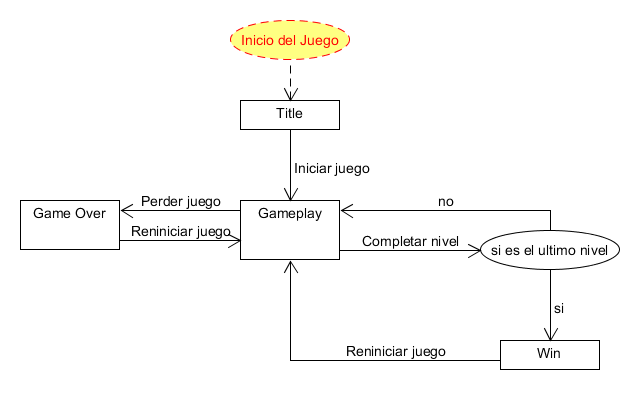
\includegraphics[width=0.8\textwidth]{images/estructura/clases/scenes}
	\centering
	\caption{Diagrama de las escenas del juego}
\end{figure}
  
\subsection{GameObjects, Componentes y Prefabs}
En Unity, los nodos de escena son implementados mediante la clase \textbf{GameObjects}. El concepto de los GameObject es uno de los más importantes a la hora de trabajar con Unity\cite{unity_manual}, ya que todos los objetos que el programador puede crear usando el editor de grafico pertenecen a esta clase. Sin embargo, la clase en si misma carece de funcionalidad. La funcionalidad viene dada de la adición de Componentes a los GameObjects, los cuales les otorgan distintas propiedades. Los componentes son un patrón de diseño muy utilizado permite desacoplar el código de los programas manteniendo la posibilidad de crear entidades con mucha funcionalidad\cite{game_programming_patterns}.

Unity incluye un gran número de componentes por defecto, como los \textit{Colliders} que se utilizan en la detección de colisiones, los \textit{Renderers} que permiten asignar modelos y texturas a los GameObjects o los \textbf{Audio Emitters} con los que se puede emitir música y sonido.

De estos componentes por defecto destaca el \textbf{Transform}. Este componente sirve para almacenar y manipular la información relativa a la posición, rotación y escala de los GameObjects. Un \textit{Transform} puede tener asignado otro \textit{Transform} a modo de padre, creando estructuras jerárquicas en las que los cambios de posición rotación y escala del padre se aplican también al hijo. Debido a que su funcionalidad es muy común y necesaria, este componente está incluido por defecto a todos los GameObjects.

Para la creación de nuevos componentes (llamados Scripts por Unity), el programador debe utilizar uno de los dos posibles lenguajes de programación soportados por Unity: \textbf{C\#,} un lenguaje de programación orientado a objetos desarrollado originalmente por Microsoft para su framework; y \textbf{UnityScript}, un lenguaje basado en JavaScript creado específicamente para Unity. Para este proyecto se optó por usar C\#.

\begin{figure}[h]
	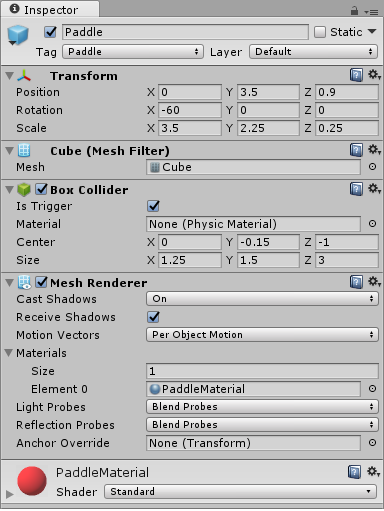
\includegraphics[width=0.5\textwidth]{images/estructura/clases/inspector}
	\centering
	\caption{Inspector de objetos mostrando los componentes del objeto \textit{Paddle}}
\end{figure}

Para que los scripts puedan funcionar como componentes, es necesario que sus clases hereden de la clase \textbf{MonoBehaviour} que incluye Unity. Esta clase contiene la funcionalidad necesaria para los componentes, como métodos de acceso a las propiedades del GameObject o funciones que son llamadas por Unity cuando ocurren ciertas acciones dentro del juego, como \textbf{Start}, que es llamado cuando crea el GameObject o \textbf{Update} que se llama una vez por cada fotograma del juego.

La creación de instancias de GameObjects, así como la asignación de componentes a estos se puede realizar tanto de forma gráfica mediante el editor de Unity como por código de programación. Como este proceso es muy lento y laborioso (especialmente realizándolo por código), Unity ofrece la posibilidad de crear múltiples GameObjects con el mismo conjunto componentes adheridos mediante el uso los Prefabs. Los prefabs son un tipo de Assets basados en el patrón de programación \textit{Prototype}\cite{game_programming_patterns} permite guardar GameObjects con componentes adheridos para poder generar copias a partir de él, tanto en el editor como por código en tiempo de ejecución. 

\subsection{Estructura de Clases}
A continuación, se encuentra una gráfica con la estructura de clases del proyecto. Aclaramos que solo se incluyen las clases creadas expresamente para este proyecto concreto, ignorando las clases incluidas por defecto en Unity o por librerías externas utilizadas. También se han resumido sus atributos y métodos para facilitar la lectura.

\clearpage 
La estructura de clases es la siguiente:
\begin{figure}[h]
	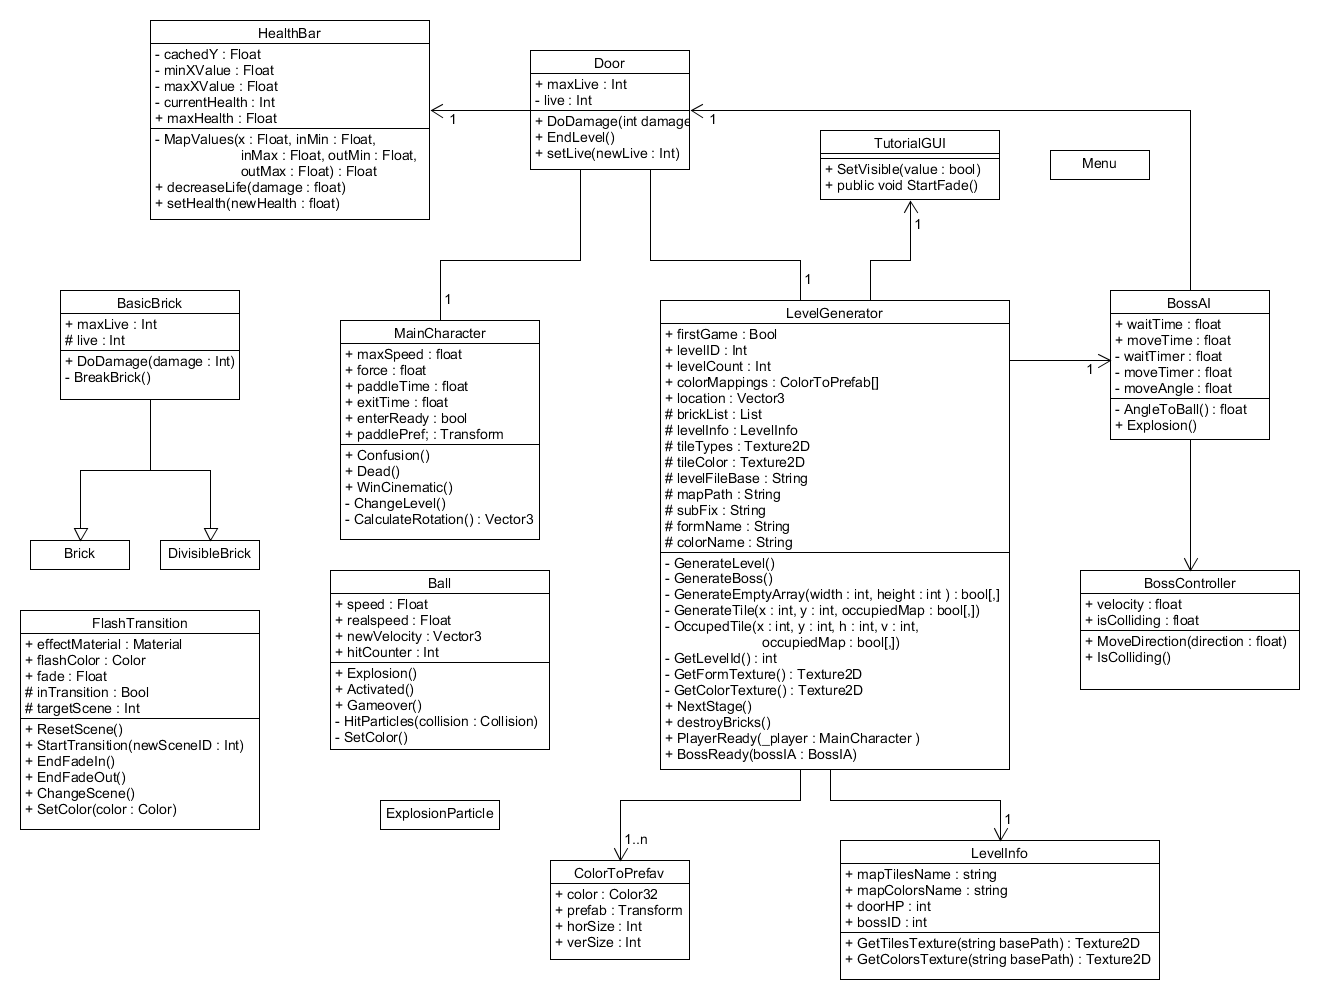
\includegraphics[width=1\textwidth]{images/estructura/clases/classes}
	\centering
	\caption{Estructura de clases}
\end{figure}

\subsection{Prefabs}
Sin embargo, la estructura de clases del juego no tiene mucho sentido por si misma si no se conoce como se asocian entre sí para formar GameObjects. Por ese motivo, en este apartado vamos a mostrar la colección de gameObjects que se utiliza en las distintas escenas del juego.

\clearpage 
En primer lugar, la escena principal (donde se desarrolla la acción del juego) cuenta con los siguientes GameObjects:
\begin{figure}[h]
	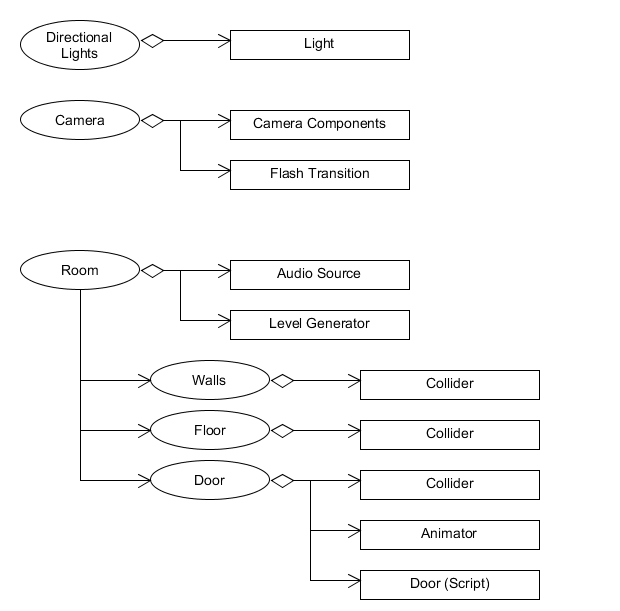
\includegraphics[width=1\textwidth]{images/estructura/clases/room-objects-1}
	\centering
\end{figure}
\begin{figure}[h]
	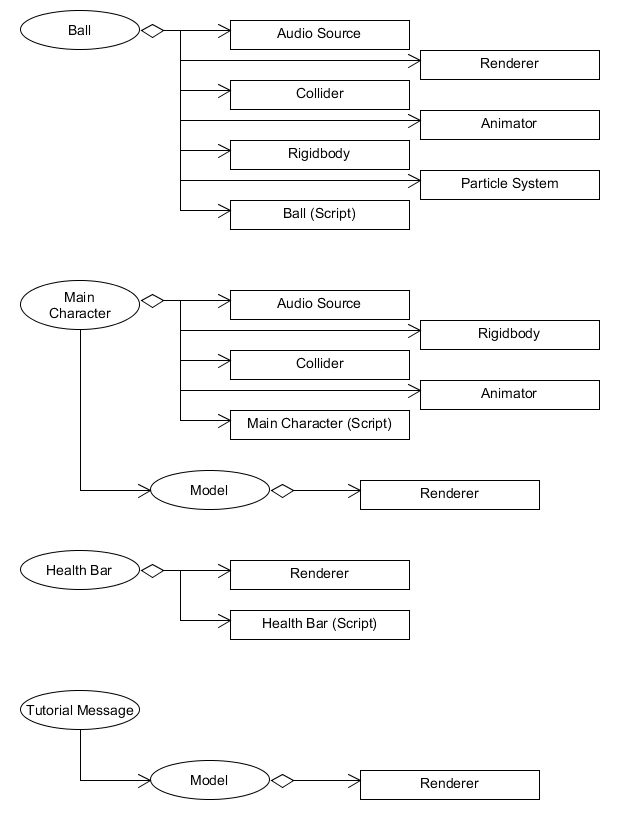
\includegraphics[width=1\textwidth]{images/estructura/clases/room-objects-2}
	\centering
	\caption{Lista de GameObjets en la escena principal}
\end{figure}

\clearpage 
A estos GameObjects hay que añadirles una serie de Prefabs adicionales que no se encuentran en escena al inicio de la ejecución, pero son añadidos de forma dinámica cuando son necesarios. Estos prefabs son:
\begin{figure}[h]
	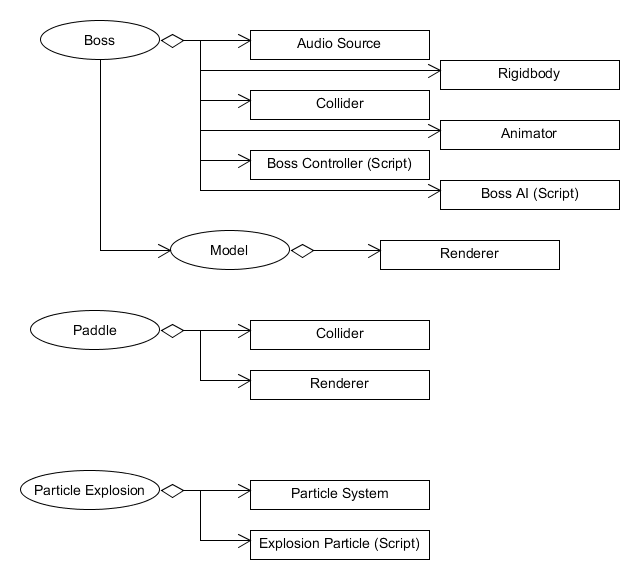
\includegraphics[width=1\textwidth]{images/estructura/clases/room-prefab-1}
	\centering
\end{figure}

\begin{figure}[h]
	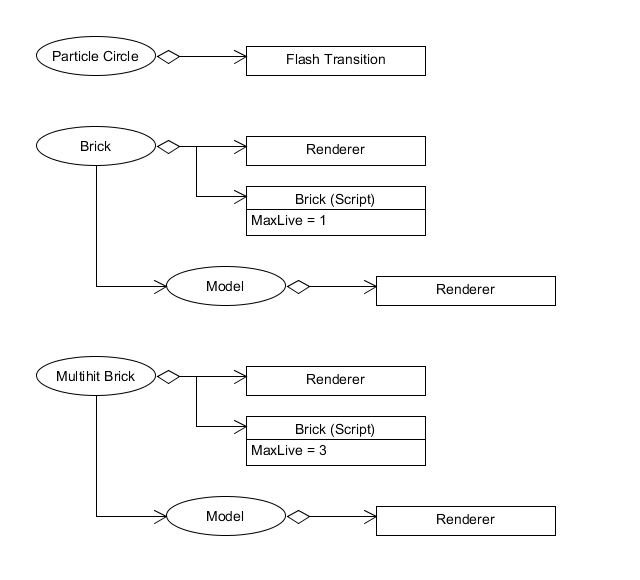
\includegraphics[width=1\textwidth]{images/estructura/clases/room-prefab-2}
	\centering
\end{figure}

\begin{figure}[h]
	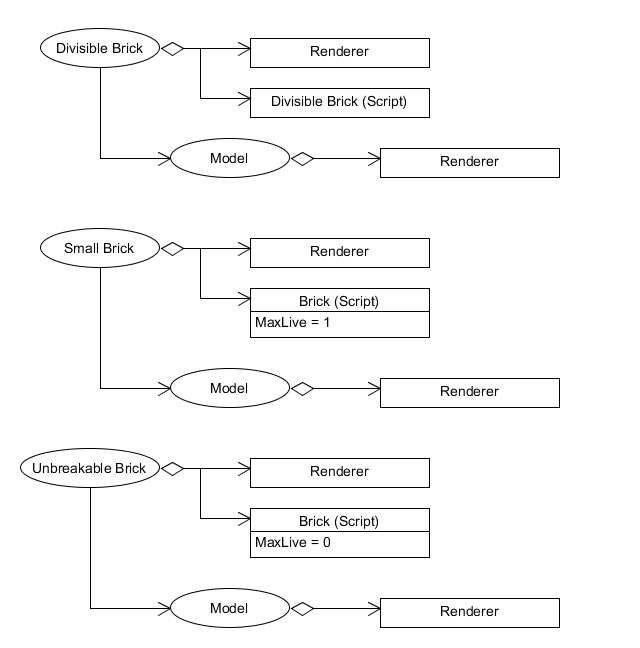
\includegraphics[width=1\textwidth]{images/estructura/clases/room-prefab-3}
	\centering
	\caption{Prefabs de la escena Principal}
\end{figure}

\clearpage 
Finalmente, la pantalla de título y final del juego cuentan con sus propios GameObjects (solo se mostrará una gráfica dado que la estructura de ambas escenas es prácticamente idéntica). Los GameObjects de estas escenas son:
\begin{figure}[h]
	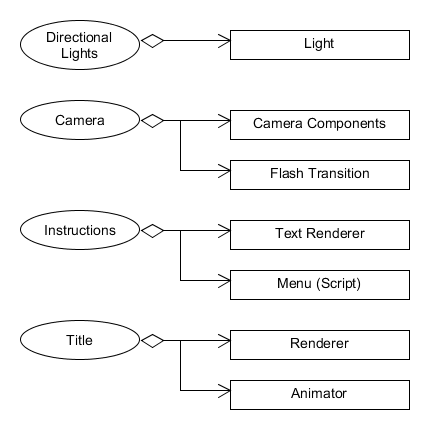
\includegraphics[width=0.65\textwidth]{images/estructura/clases/title-objects}
	\centering
	\caption{Lista de GameObjets en los menús}
\end{figure}

\clearpage 
\section{Carga y Estructura de Niveles}
El diseño de los distintos niveles del juego fue un punto muy importante del desarrollo. Desde un principio se tenía claro que había que minimizar todo lo posible el tiempo que se requeriría para trasladar el diseño de un nivel a su complementación en Unity. Basándose en los requisitos de los niveles de este género de juego, las principales capacidades que se deseaban para el editor eran las siguientes:

\begin{itemize}
  \item Precisión: Poder alinear los bloques con una cuadricula de forma automática, para así mantener la estética de juego ``retro'' deseada.
  \item Facilidad para añadir y eliminar niveles sin tener que modificar el código del juego. 
  \item Posibilidad de elegir individualmente e color para cada uno de los bloques del nivel, independientemente de su comportamiento o posición. Esto nos permite decorar los niveles y hacerlos más memorables para el jugador. 
  \item Simplicidad en el proceso de creación. En la medida de lo posible, la creación de niveles deberá poder hacerse de forma gráfica, sin escribir código.
\end{itemize}

\begin{figure}[h]
	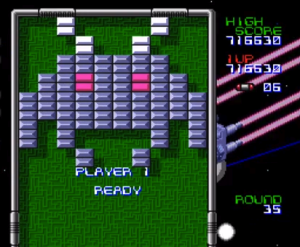
\includegraphics[width=0.7\textwidth]{images/estructura/niveles/ejemplo-arkanoid}
	\centering
	\caption{Homenaje a Space Invaders(Taito, 1978) dentro de Arkanoid: Doh it Again (Taito, 1997)}
\end{figure}

Tras una primera iteración en la que los niveles se implementaban en el propio editor de escenas de Unity, se optó por utilizar Tiled. Tiled es un editor de mapas de propósito general que permite editar mapas basados en baldosas o ``Tiles''. Los mapas desarrollados generados con Tiles eran exportados al formato XML, el cual podía se cargado en Unity. Sin embargo, la producción de niveles era demasiado lenta debido a determinadas carencias en el programa, lo que nos llevó a replantear el sistema.

El nuevo enfoque se basa en la lectura de pequeñas imágenes que contienen la información del nivel codificada en los colores de sus pixeles. En este sistema toma dos imágenes para generar el nivel. La primera imagen sirve para determinar el tipo y posición de los bloques, mientras que la segunda imagen determina los colores de cada bloque. Un archivo JSON adicional sirve para ``enlazar'' ambas imágenes y para contener información adicional, como la cantidad de golpes que debe recibir la puerta para abrirse o de si debe iniciarse o no un combate de jefe.

El sistema de carga de niveles está implementado en la clase LevelGenerator, un componente adherido al objeto Room. El proceso de carga de niveles funciona así:
\begin{enumerate}
  \item Se lee el archivo JSON determinado por el índice del nivel actual. La lectura del archivo se realiza mediante la clase JsonUtility de Unity, que automáticamente genera un objeto con la estructura contenida el archivo JSON.
  \item El sistema determina si se trata de un nivel de jefe. En ese caso se detiene el proceso y se empieza a preparar la batalla con el jefe. En caso contrario, se continua con el proceso.
  \item Se cargan las imágenes del nivel en forma de dos texturas de la clase Texture2D. A efectos prácticos, cada textura es una matriz bidimensional de objetos Color. Llamaremos Textura de tipos a aquella que determina el tipo de los bloques y Textura de colores a aquella que determina sus colores.
  \item Se recorre la textura de tipos obteniendo los valores de sus pixeles. Cada pixel se compara con una tabla de equivalencias que relaciona un tipo de bloque con un color. En caso de acierto, se instancia un bloque del tipo determinado, al cual se asigna el color del pixel de la textura de colores de la misma posición.
  \item Dado que los bloques ocupan más de una ``casilla'', cada vez que uno es creado se marcan las posiciones que ocupan en una ``matriz de ocupación''. durante el recorrido de la textura, se ignorarán los pixeles que correspondan a posiciones ocupadas.
  \item Finalmente, se asigna el número de golpes que requiere la puerta.
\end{enumerate}

De esta forma es posible producir niveles rápidamente, los cuales son fáciles de modificar. La implementación del sistema está realizada de forma que es capaz de ``ignorar'' pequeños errores en el mapa, como asignación de colores a casillas vacías o la presencia de colores que no se corresponden con ningún tipo de bloque.

Sin embargo, este sistema no está exento de limitaciones:
\begin{itemize}
  \item En primer lugar, solo una pequeña cantidad de estos pueden ser asignados a tipos de bloques. Esto se debe a las discrepancias entre los formatos de colores (los componentes RGB de los colores se guardan como enteros entre 0 y 255 en las texturas, pero como números de punto flotante entre 0 y 1 en la clase Color), la cual provoca perdida de información durante la conversión y nos fuerza a utilizar valores de color que sean fracciones exactas de 256. 
  \item En segundo lugar, se trata de un sistema poco escalable, permitiendo un tamaño único de campo de juego y poca capacidad para ``personalizar'' los tipos de bloque más allá de su color; por lo que sería necesario realizar cambios importantes en caso de que se necesitaran construir niveles más complejos
\end{itemize}

\section{Control de movimiento y físicas}
Los videojuegos son por definición sistemas interactivos en los que uno o más elementos de este reaccionan a las acciones del jugador. En nuestro caso, los dos elementos móviles que se encuentran a disposición del jugador son el personaje principal y la pelota.

El movimiento de estas dos entidades se implementó haciendo uso del motor de físicas incluido dentro de Unity Engine, el motor PhysX de Nvidia\footnote{https://developer.nvidia.com/unity}. El uso de un motor de físicas permitió agilizar el desarrollo ya que incluye mucha funcionalidad necesaria para el funcionamiento del juego, como la detección de colisiones, el movimiento con aceleración y desaceleración, la simulación de gravedad o el efecto de rebote de cuerpos en movimiento.

El comportamiento de las dos entidades se controla internamente mediante una máquina de estados finitos. El uso de este patrón de programación facilitó enormemente el desarrollo de estos objetos, ya que permitía controlar de forma precisa como iban a reaccionar las entidades en cada momento y reducía enormemente el tamaño de las lógicas de control, evitando así fallos difíciles de detectar\cite{game_programming_patterns}. La implementación de la máquina de estados finitos se implementó mediante la librería \textit{Simple Finite State Machine} de \textit{Made With Monster Love}\footnote{https://github.com/thefuntastic/Unity3d-Finite-State-Machine}

En los siguientes apartados describiremos en detalle la implementación de las dos entidades


\subsection{Personaje principal}
El personaje principal es el avatar del jugador en el juego, al que controla directamente mediante el teclado. Su comportamiento es bastante sencillo: el personaje se mueve cuando el jugador pulsa las flechas de dirección, y crea una ``paleta'' cuando se pulsa la tecla espacio. Usando la paleta, el personaje es capaz de redirigir la pelota, pero si la pelota impacta contra el directamente se quedará aturdido unos segundos. La paleta solo permanece activa unos instantes, en los cuales el personaje permanece inmóvil, por lo que presenta un desafío para el jugador, que debe saber posicionarse correctamente. El personaje reproduce también una animación al inicio de los niveles y otra al final, en la que entra y sale de la sala del juego.

\begin{figure}[h]
	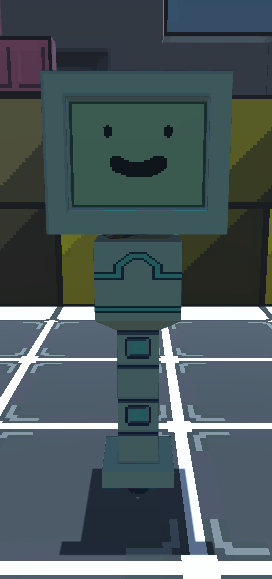
\includegraphics[width=0.30\textwidth]{images/estructura/fisica/flick_happy_small}
	\centering
	\caption{Modelo del personaje principal}
\end{figure}

Los estados que componen al personaje principal son los siguientes:
\begin{itemize}
	\item \textbf{Enter}: Es el estado inicial. En este estado el personaje, posicionado fuera de escena, se mueve hacia el interior de la sala hasta colocarse en el centro de esta. Durante este estado, la colisión y la gravedad están desactivadas, lo que le permite entrar en la sala cerrada. Una vez terminada la animación, pasa al estado \textbf{Stand}.
  	\item \textbf{Stand}: Se trata del estado principal. En él, el personaje espera inmóvil a recibir las órdenes del personaje. Si se pulsan las flechas de dirección, el personaje pasará al estado \textbf{Move} y si se pulsa la tecla espacio, se pasará al estado \textbf{Paddle}.
	\item \textbf{Move}: En este estado el personaje se mueve a velocidad constante en la dirección determinada por las flechas pulsadas. Cuando ninguna de las flechas de dirección esté siendo pulsadas, se volverá al estado \textbf{Stand}. En este estado también se puede pulsar la tecla espacio para moverse entrar en el estado \textbf{Paddle}.
	\item \textbf{Paddle}: En este estado el personaje crea frente a el un objeto Paleta que sirve para desviar la pelota. La paleta tiene un temporizador que hace que, al acabarse, la paleta desaparezca y el personaje vuelve al estado \textbf{Stand}. Durante este estado el jugador no se puede mover, aunque si se entró desde el estado \textbf{Move} todavía se conservará parte de la velocidad debido a la inercia.
	\item \textbf{Confused}: El personaje entra en este estado cuando la pelota le golpea, independientemente de en qué estado se encuentre. En este estado, el jugador girará aturdido durante unos instantes antes de volver al estado \textbf{Stand}, como penalización para el jugador por no haber golpeado la pelota correctamente.
	\item \textbf{Dead}: El personaje entra en este estado cuando la pelota es destruida, sin importar el estado anterior. En este estado el personaje se desploma derrotado y se queda inmóvil, a espera de la pantalla de ``fin del juego''.
    \item \textbf{Exit}: Cuando se completa un nivel, el personaje entra en este estado. El estado tiene dos partes: primero, el personaje permanece inmóvil a la espera de que la puerta del nivel se abra; y una vez esta esté abierta, el personaje avanza a través de ella hacia el siguiente nivel.
\end{itemize}

\begin{figure}[h]
	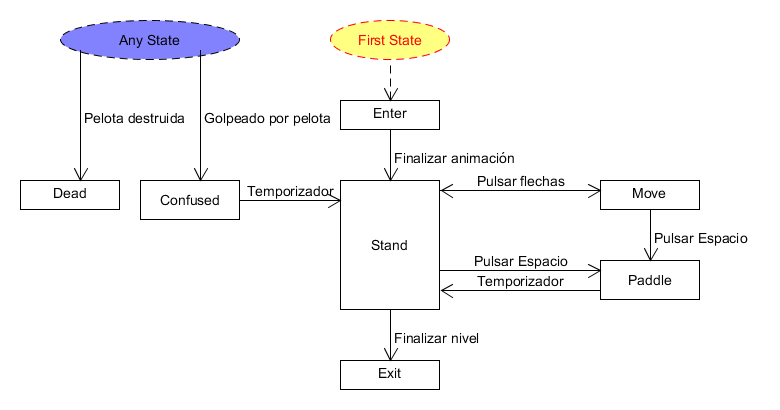
\includegraphics[width=0.8\textwidth]{images/estructura/fisica/player}
	\centering
	\caption{Diagrama de estados del personaje principal}
\end{figure}

Los movimientos del personaje (tanto durante el movimiento controlados por el jugador como durante las animaciones de principio y final del nivel) se implementaron mediante el uso de fuerzas del sistema de físicas. Esto hacía que el jugador se moviese de forma fluida sin cambios bruscos de velocidad. Para el movimiento controlado por el jugador, se utilizaron fuerzas muy grandes en conjunción con un factor de fricción también elevado, lo que permitía controlar al personaje con precisión. Esto se combina con una reducción de la fricción en el estado \textbf{Paddle} para que el personaje conservase parte de su velocidad al sacar la paleta, lo que servia para aumentar el margen de error del jugador a la hora de intentar golpear la pelota.

\begin{figure}[h]
	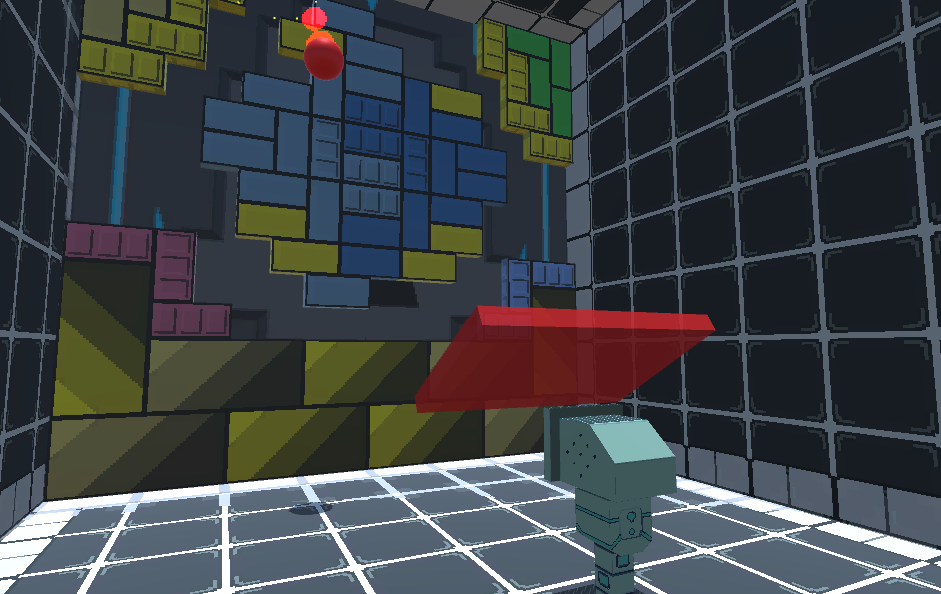
\includegraphics[width=0.8\textwidth]{images/estructura/fisica/flick_paddle}
	\centering
	\caption{Personaje principal activando la paleta}
\end{figure}

Las animaciones del personaje se realizaron mediante el motor de animaciones de Unity. Este motor permite animar los elementos del juego alterando sus propiedades (como la posición, rotación y escala de los modelos) durante intervalos de tiempo. El sistema funciona como una máquina de estados que permite cambiar entre distintos ``clips'' de animación dependiendo de variables de control de los objetos. Las animaciones que se crearon para el personaje son muy sencillas (cambios de escala y rotación) por lo que no hicieron uso de las propiedades más avanzadas del motor de animaciones (como los arboles de mezcla de animación\footnote{https://docs.unity3d.com/Manual/class-BlendTree.html} o la cinemática inversa\footnote{https://docs.unity3d.com/Manual/InverseKinematics.html})

\subsection{Pelota}
Podríamos considerar la pelota como el ''arma'' del personaje principal, el medio por el que el jugador interacciona con los objetos del juego. La pelota viaja en trayectoria rectilínea, rebotando en las paredes y el techo de la sala del juego. Al golpear la puerta, o los bloques que la cubren, estos reciben daño y la pelota rebota, pero si la pelota golpea el suelo de la sala es la pelota la que recibe daño. Si la pelota golpea el suelo tres veces, se acaba la partida. El jugador debe intentar golpear la pelota con la paleta para redirigirla hacia la puerta, evitando que toque el suelo.

\begin{figure}[h]
	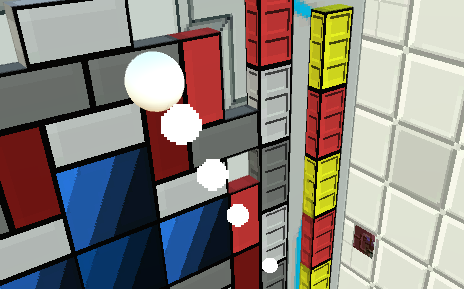
\includegraphics[width=0.65\textwidth]{images/estructura/fisica/ball_moving}
	\centering
	\caption{Pelota moviéndose}
\end{figure}

La máquina de estados de la pelota es significativamente más simple que la del personaje jugador, contando solo con tres estados: \textbf{Normal} (su comportamiento normal de movimiento), \textbf{Destroy} (animación de destrucción de la pelota que se reproduce al final del juego) y \textbf{Locked} (estado especial en el que la pelota permanece quieta e invisible, para la cinemática de inicio y final del nivel).  Sin embargo, la tabla de interacciones de la pelota es mucho más extensa, debido a que tiene una reacción distinta para cada objeto del juego con el que colisione. Las posibles reacciones son:
\begin{itemize}
	\item Al golpear la \textbf{Puerta} de la sala los \textbf{Bloques} que la cubren, estos sufrirán un punto de daño, y la pelota rebotará. Al iniciarse el rebote, la pelota empezará a caer en dirección al suelo de la sala.
	\item Al golpear las \textbf{Paredes} o el \textbf{Techo} de la sala, la pelota rebotará de forma natural.
	\item Al golpear el \textbf{Suelo} de la sala, la pelota recibirá un punto de daño. Además, la pelota rebotará, pero no de forma natural sino de forma que vaya en dirección a la puerta. Esto sirve principalmente para facilitar la tarea del jugador, ``regalándole'' un golpe a la puerta. La pelota también pierde la fuerza de la gravedad.
	\item Al golpear al \textbf{jugador}, este se quedará aturdido unos instantes y la pelota rebotará de forma natural.
	\item Al golpear la paleta del jugador, la pelota rebotará y perderá la fuerza de la gravedad. La dirección en la que rebotará la pelota dependerá del punto de la paleta en el que golpeó la pelota, siendo la dirección normal al plano de la paleta si se golpea justo en el centro.
\end{itemize}
\begin{figure}[!htb]
   \begin{minipage}{0.5\textwidth}
     \centering
     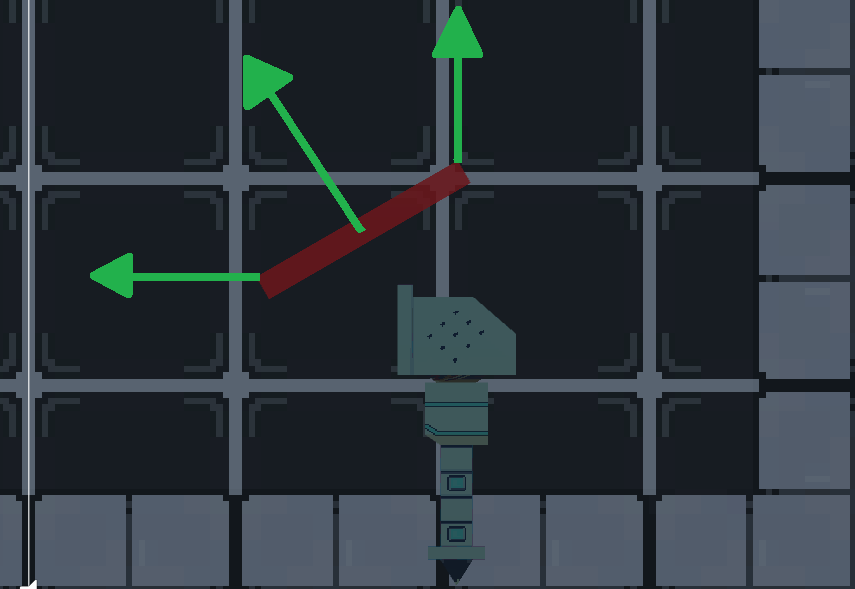
\includegraphics[width=0.9\linewidth, right]{images/estructura/fisica/paddle_direction_side}
   \end{minipage}\hfill
   \begin {minipage}{0.5\textwidth}
     \centering
     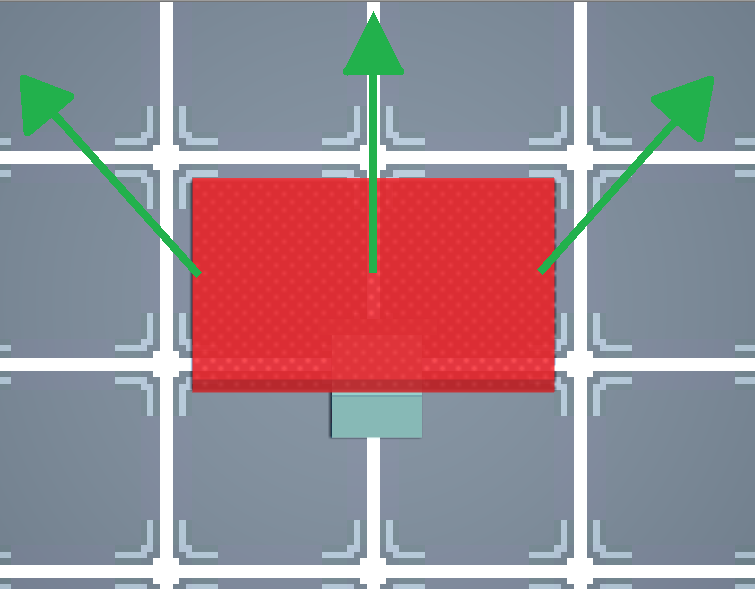
\includegraphics[width=0.9\linewidth, left]{images/estructura/fisica/paddle_direction_top}
   \end{minipage}
   \caption{Direcciones que tomaría la pelota dependiendo del punto de la paleta que golpee (Aproximada)}
\end{figure}
El movimiento de la pelota se basa íntegramente el motor de físicas de Unity. Al entrar en su estado \textbf{Normal}, la pelota recibe un impulso en una dirección dada y a partir de ahí se moverá sin fricción   de forma perpetua. Los movimientos ``antinaturales'' mencionados, el cambio de dirección al golpear el suelo o la paleta se realizan cambiando el vector de la velocidad de la pelota por un vector nuevo generado manualmente por código.

Aunque la pelota no tiene animación en si misma, a su comportamiento se le han añadido unos efectos de partículas creados mediante el motor de partículas de Unity\footnote{https://docs.unity3d.com/Manual/ParticleSystems.html}, que sirven tanto para embellecer el juego como para crear guías visuales para el jugador. La pelota cuenta con tres efectos animados de partículas: una ``cola'' que marca la trayectoria que siguió la bola; un efecto circular que aparece cuando la bola colisiona con las paredes, el techo y el suelo, que sirven para marcar el punto de impacto de la bola y un efecto de explosión final.
\begin{figure}[!htb]
   \begin{minipage}{0.48\textwidth}
     \centering
     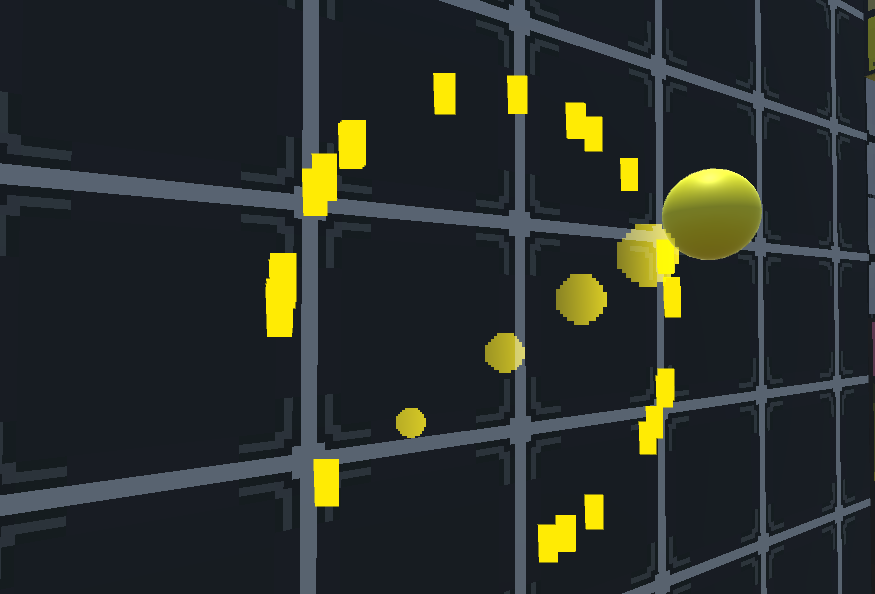
\includegraphics[width=0.7\linewidth, right]{images/estructura/fisica/ball_hit}
   \end{minipage}\hfill
   \begin {minipage}{0.48\textwidth}
     \centering
     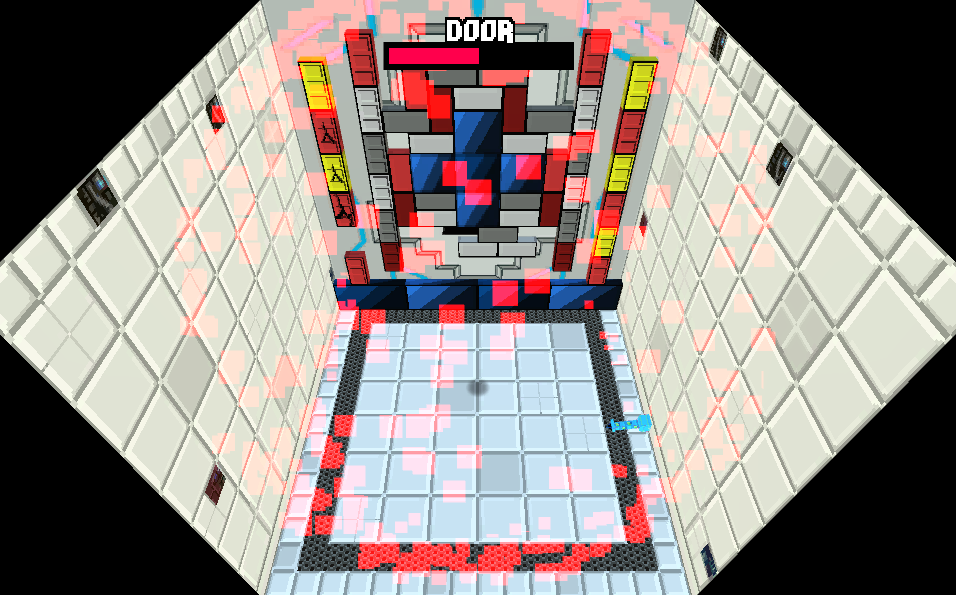
\includegraphics[width=0.7\linewidth, left]{images/estructura/fisica/ball_explosion}
   \end{minipage}
   \caption{Efectos de partículas: impacto en muro (izquierda) y explosión (derecha)}
\end{figure}

\section{Jefe Final}
Un jefe final, o monstruo jefe, es un enemigo poderoso al que los jugadores deben enfrentarse para poder alcanzar algún objetivo dentro del juego \cite{game-design-patterns}. Los jefes sirven principalmente para tres propósitos: dar clausura a una sección del juego, al colocarse al final de una sección, nivel o fase; ofrecen variedad al juego, al suponer una variación con respecto al juego corriente y finalmente sirven como ``test'' para el jugador, al tratarse de un desafió mucho mayor que los anteriores. 

Para este juego, el jefe final es el único ``enemigo'' al que se enfrenta el jugador, que aparece en el nivel 11 del juego. Este jefe se comporta como un ``clon'' o ``rival'' del jugador: su objetivo es impedir que la pelota golpee la puerta, moviéndose y redirigiéndola de forma similar a como lo haría el jugador. El jefe se mueve a velocidad constante, siempre pegado a la pared, en dirección a la pelota cuando detecta que esta se mueve hacia la pared. Para evitar que este enemigo sea imbatible, su velocidad se reduce cada vez que consigue la pelota, lo que provoca que se vuelva incapaz de seguirle el ritmo a esta después de un tiempo.

\begin{figure}[h]
	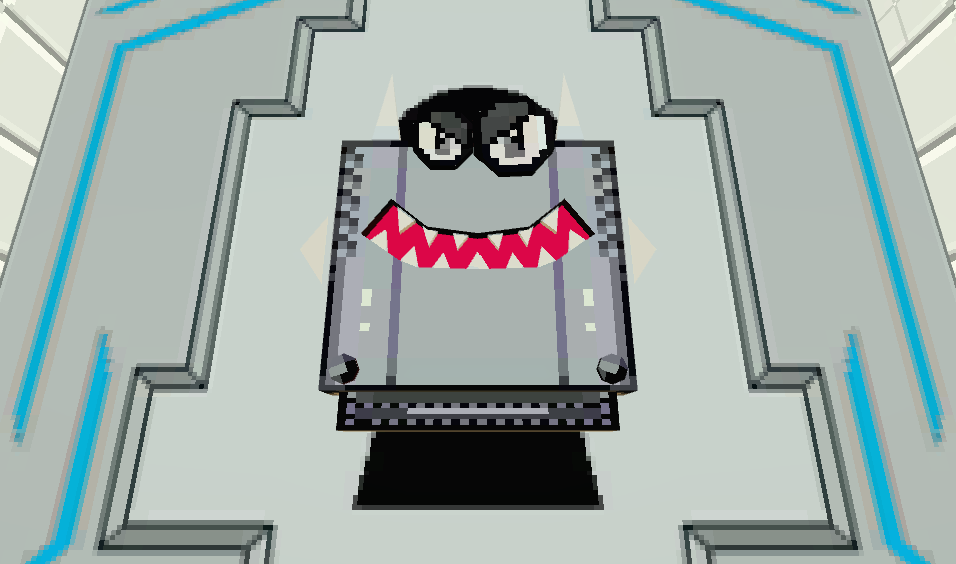
\includegraphics[width=0.30\textwidth]{images/estructura/jefe/boss-captura}
	\centering
	\caption{Modelo del Jefe.}
\end{figure}

La forma de derrotar a este jefe es idéntica de a como se supera cualquier fase: Golpeando la puerta suficientes veces.

\subsection{Implementación}
La implementación de este jefe se realizó usando el sistema de Prefabs y Componentes de Unity. El jefe es un Prefab al que el sistema de carga de niveles instancia en los niveles marcados como niveles de jefe. Este Prefab está formado por dos GameObjects: el primero, que se encarga de determinar el comportamiento del jefe y un GameObject hijo que contiene el modelo del jefe. Se implementa de esta para permitir cambios en el modelo del jefe sin que se tenga que ajustar el comportamiento y también para facilitar la animación. El GameObject principal, por otro lado, incluye una serie de componentes que se encargan de modelar distintas partes su comportamiento. La mayor parte de estos son componentes por defecto de Unity:
 \begin{itemize}
	\item \textbf{Transform}: Almacena la posición, rotación y escala del jefe, información básica de todo objeto del juego. 
	\item \textbf{Collider}: Se utiliza en la detección de colisiones.
	\item \textbf{Rigidbody}: Otorga propiedades físicas al GameObject, como velocidad, masa o aceleración. Simplifica enormemente la implementación del movimiento del jefe.
	\item \textbf{Animator}: Permite añadir animaciones al GameObject, las cuales alteran las propiedades de sus componentes basándose en el tiempo. Se utiliza para crear dotar al jefe de animaciones sencillas de modo que no resulte demasiado estático.
	\item \textbf{Audio Source}: Sirve para emitir sonidos y música. El jefe lo utiliza para emitir sonidos en situaciones concretas, como al golpear la pelota o al ser derrotado.
\end{itemize}

\begin{figure}[h]
	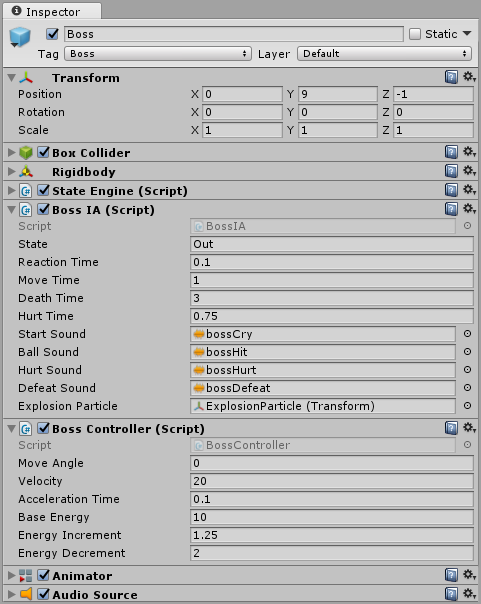
\includegraphics[width=0.5\textwidth]{images/estructura/jefe/boss-component}
	\centering
	\caption{Inspector mostrando los componentes del Jefe.}
\end{figure}

Para controlar el comportamiento del jefe se implementaron también dos scripts: \textbf{BossController} y \textbf{BossAI}. \textbf{BossController} Contiene la información y las funciones necesarias para facilitar el movimiento del jefe. El método principal de esta clase, \textit{MoveDirection()}, permite mover al jefe a velocidad constante en el ángulo suministrado, siempre en relación con el plano de la puerta. El movimiento se implementa a través del Componente Rigidbody, aplicando fuerza constante en la dirección indicada, lo que crea un movimiento con una ligera aceleración que resulta más natura que un cambio instantáneo de velocidad. El script implementa también un sistema de energía: cuanto mayor sea la energía, más rápido se mueve.

Este método es utilizado por el segundo script, \textbf{BossAI}, para mover al jefe. El script \textbf{BossAI} codifica el comportamiento del jefe en forma de una máquina de estados finitos que decide la forma en la que el jefe se mueve dependiendo de la dirección de la bola. También se encarga de aumentar y reducir la energía del jefe y de cambiar la animación. El comportamiento se compone de los siguientes estados:
 \begin{itemize}
	\item \textbf{Out}: El jefe espera fuera del área de juego, inmóvil, a la espera de la entrada del jugador en la sala.
	\item \textbf{Intro}: El jefe se mueve a su posición inicial y realiza su animación inicial. Este movimiento se implementa mediante el uso de animaciones en lugar de mediante el BossController dado que debe atravesar las paredes de la sala.
	\item \textbf{Wait}: En este estado, el jefe permanece inmóvil a la espera de un estimulo que le haga cambiar iniciar el movimiento, en concreto, que se detecte que la pelota se aproxima a la puerta.
	\item \textbf{Move}: El jefe se mueve en dirección a la pelota utilizando los métodos de BossController. El movimiento se detendrá si se consigue golpear la pelota o si la pelota golpea la puerta. 
	\item \textbf{Hurt}: En este estado el jefe permanece inmóvil mientras se reproduce una animación de daño. Tras esta breve pausa, el jefe retorna al estado Wait.
	\item \textbf{Death}: Cuando la puerta se abre, el jefe realiza una animación de destrucción, en la que el jefe se vuelve invisible y emite una explosión de partículas. 
\end{itemize}

\begin{figure}[h]
	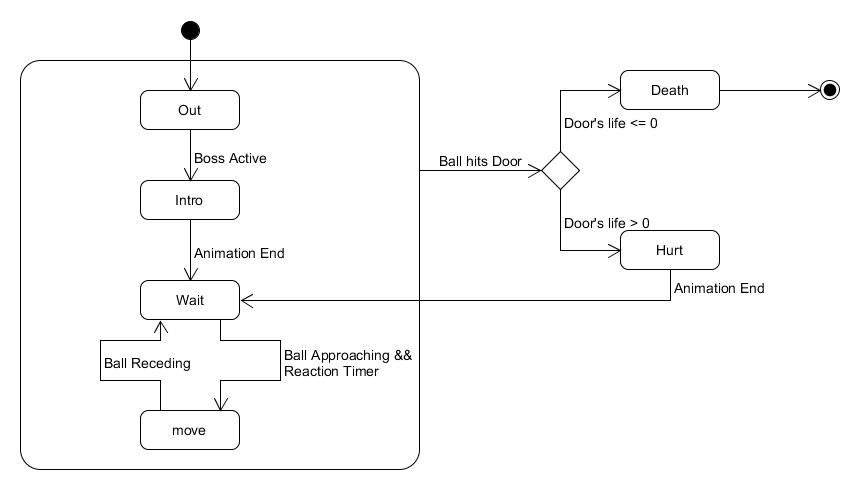
\includegraphics[width=0.9\textwidth]{images/estructura/jefe/boss-estados}
	\centering
	\caption{Diagrama de estados del jefe.}
\end{figure}

Cuando la pelota golpea al jefe, este cambia la dirección de la pelota. Esta redirección no sigue el ángulo ``natural'' que seguiría la pelota si ``rebotase'' contra el jefe, sino que es redirigido hacia el jugador. El propósito de este comportamiento es crear una situación en la que el jefe y el jugador se intercambian la pelota como si de un partido de tenis se tratase. Cada vez que la pelota golpea al jefe, BossIA reduce la energía de BossController. 

Por otro lado, si el jefe falla al golpear la pelota, y esta golpea la puerta, BossIA restaurará la energía y aumentará por encima del máximo inicial, incrementando el la velocidad. Esto provoca un incremento progresivo de la dificultad a medida que avanza el combate.

El objetivo de este diseño en dos componentes del comportamiento del jefe nos permite mantener una separación entre la implementación del movimiento y el comportamiento propiamente dicho. De esta forma, podremos remplazar, por ejemplo, la inteligencia artificial por un controlador manual para implementar un modo de dos jugadores, o usar el módulo de la inteligencia artificial en otro jefe distinto cuyo comportamiento se base también en la posición de la bola.
